%%%%%%%%%%%%%%%%%%%%%%%%%%%%%%%%%%%%%%%%%%%%%%%%%%%%%%%%%%%%%%%%%%%%%%%%%%%%%%%%
% Touch Settings
%%%%%%%%%%%%%%%%%%%%%%%%%%%%%%%%%%%%%%%%%%%%%%%%%%%%%%%%%%%%%%%%%%%%%%%%%%%%%%%%
\chapter{Touch Settings} \label{Touch Settings}
\vspace{-10ex}\mTS{syml}\vskip 8ex

%%%%%%%%%%%%%%%%%%%%%%%%%%%%%%%%%%%%%%%%%%%%%%%%%%%%%%%%%%%%%%%%%%%%%%%%%%%%%%%%
% Introduction
%%%%%%%%%%%%%%%%%%%%%%%%%%%%%%%%%%%%%%%%%%%%%%%%%%%%%%%%%%%%%%%%%%%%%%%%%%%%%%%%
\section{Introduction}

Allows for configuring, calibrating and testing the touch sensing capability of
the device.  It can also be disabled here.

\par\medskip

In this mode, the main goal is to come up with a number called a touch
threshold.  When a reading is taken, if its value is greater than the threshold,
a touch event is registered.  It's recommended that you first select the
\mTSCa{f} menu option and follow the instructions for that.  If you are unable
to get a consistent beep without chirping when touching during \sTSTA{f}, try
the \mTSRe{f} method, then the \mTSCo{f} method.  If nothing good comes of any
of these, you can load the \mTSDe{f} and try again or simply \mTSDi{f} touch
altogether.  Most everything that can be done using touch can be done using
other means.  There are a few exceptions:

\begin{itemize}
  \item Forcibly putting the device to sleep -
    see \hyperref[Power Settings - Touch]{Touch} in
    \hyperref[Power Settings]{\mPS{f}} and \hyperref[Power - Touch]{Touch Sleep}
    in \hyperref[Power]{\mPo{f}}.
  \item Toggling the timer lighting - see \hyperref[Timer - Lighting]{Lighting}
    in \hyperref[Timer]{\mTi{f}}.
\end{itemize}

There are a few ways to get to \mTS{f} depending on which direction the \cRs{f}
is pointing and which mode the device is currently in.  The most straightforward
way is:

\begin{enumerate}
  \item \aTu{f} the \cRs{f} to the \dLe{f}.
  \item \aPH{f} the \cEs{f} until \symD{>>>>} is blinking on the
    \cDi{f} then \aRe{f}.
\end{enumerate}

\begin{table}[H]
\ers{1}
\centering
\begin{tabu} { X[1,c,m] | X[2,c,m] | X[1,c,m] }
  \thrule
  \thbi{Position} & \thbi{Mode} & \thbi{Action} \\ \mrule

  \sMi & \multirow{2}{*}[-1.5mm]{\mode{s}{ANY}}
    & $\hskip -5mm$ \sMtoL \\ \dcrule{1}{1} \dcrule{3}{3}
  \sRi & & \sRtoL \\ \mdrule

  \multirow{2}{*}[-1.5mm]{\sLe} & \mSA{sym}
    & \multirow{2}{*}[-1.5mm]{\sTer} \\ \dcrule{2}{2}
    & \mSC{sym} & \\ \dcrule{2}{2}

  \bhrule
\end{tabu}
\caption{Touch Settings - Mode}
\end{table}

%%%%%%%%%%%%%%%%%%%%%%%%%%%%%%%%%%%%%%%%%%%%%%%%%%%%%%%%%%%%%%%%%%%%%%%%%%%%%%%%
% Capacitive Touch Sensing
%%%%%%%%%%%%%%%%%%%%%%%%%%%%%%%%%%%%%%%%%%%%%%%%%%%%%%%%%%%%%%%%%%%%%%%%%%%%%%%%
\section{Capacitive Touch Sensing}

The touch capability in this device uses
\href{https://en.wikipedia.org/wiki/Capacitive\_sensing}{Capacitive Touch Sensing}
which measures changes in capacitance of an \textit{electrode} to detect touch
events.  The figure below shows how it is modeled as a capacitor and the
corresponding parts of the device.

\begin{figure}[H]
\centering
  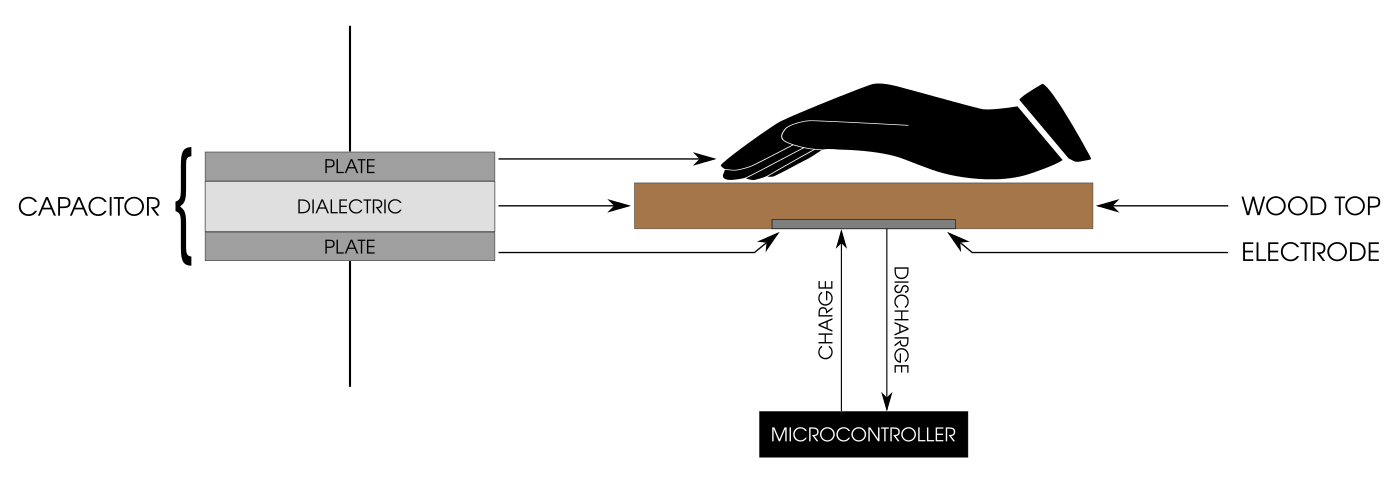
\includegraphics{images/touch_capacitive.png}
\caption{Capacitive Touch Sensing}
\end{figure}

Since humans are electrical conductors, the hand forms the other plate of the
capacitor model.  As the hand approaches and lies on top of the enclosure, the
capacitance, or charge capacity of the electrode will \textit{increase}.

\par\medskip

Changes in capacitance are detected by measuring the amount of time it takes to
charge and discharge the electrode.

\par\medskip

When a reading is taken, a fixed size reference capacitor is charged and
discharged using a configurable charge rate denoted as \sTSRC{f}.  At the same
time, the electrode is charged and discharged a set number of times using
another configurable charge rate denoted as \sTSEC{f}.  Since its capacitance
does \textit{not} change, the fixed size capacitor provides a \textit{reference} and will
always charge\slash discharge at the same rate.  On the other hand, the
electrode capacitance \textit{varies}, so its charge\slash discharge rate will
vary.  The number of times the electrode is charged\slash discharged or
\textit{scanned} per reading is determined by two configurable quantities
denoted as \sTSNS{f} and \sTSPS{f}.  \sTSNS{f} is a base
\textit{number of scans} and \sTSPS{f} is a \textit{prescaler} or multiplier
applied to \sTSNS{f}.  The product of the two determines the number of times the
electrode is charged\slash discharged during a reading.

\begin{figure}[H]
\centering
  
\includegraphics{images/touch_oscillation_graph.png}
\caption{Anatomy of a Touch Sensor Reading}
\end{figure}

As the hand approaches the electrode, the capacitance \textit{increases} resulting in
more time required to charge and discharge the electrode.  This increase in time
or decreased frequency results in more reference capacitor charges and
discharges per electrode charge\slash discharge resulting in a higher reading.

\par\medskip

As an analogy, consider the filling and draining of a bath tub - the larger the
tub, the longer it will take to fill it up and to drain it.  Think of the
electrode as a bath tub that increases in size when touched therefore taking
longer to fill and drain.  This increase in fill\slash drain time of the
electrode when touched means that the fixed size reference capacitor - a bath
tub that doesn't change in size - can be filled and drained more times per
electrode fill and drain.

\par\medskip

The \fontTGA{f}{READING} taken is basically the number of times it takes to fill
and drain the fixed size reference capacitor per electrode fill and drain cycle
- the cycle being defined as \sTSNS{f} $\times$ \sTSPS{f}.

\par\medskip

Below are two graphs that illustrate the capacitance difference and how it is
measured.  The first illustrates a reading taken when \textit{not touched} and
the second when \textit{touched}.  This example uses $\textrm{\sTSNS{f}} = 3$
and $\textrm{\sTSPS{f}} = 2$, so the number of electrode scans per reading is:
$\textrm{\sTSNS{f}} \times \textrm{\sTSPS{f}} = 6$.

\begin{figure}[H]
\centering
  
\includegraphics{images/touch_comparison_not_touched.png}
\caption{Touch Reading Comparison - Not Touched}
\end{figure}

\begin{figure}[H]
\centering
  
\includegraphics{images/touch_comparison_touched.png}
\caption{Touch Reading Comparison - Touched}
\end{figure}

When touched, the higher capacitance created means that it will take longer to
charge and discharge resulting in more reference oscillations per electrode scan
and therefore a higher reading.

\par\medskip

Despite the fact that a reading can be calculated, the device still has to be
told when a reading should be considered as a legitimate touch event.  As
initially mentioned, the main goal of \mTS{f} is to come up with a touch
\textit{threshold} value.  This is a value for which a touch event is registered
when the value of a reading equals or exceeds it.

\par\medskip

In the above example, if the threshold value was between \num{16} and \num{28}
inclusive, a touch event would \textit{not} have been registered in the
\fontTGA{f}{NO TOUCH} case and \textit{would} have been registered in the
\fontTGA{f}{TOUCH} case, as expected.

\par\medskip

However, if the threshold value was set to \num{15} or less, a touch event
\textit{would} have been registered in the \fontTGA{f}{NO TOUCH} case as well
as the \fontTGA{f}{TOUCH} case.  And if the threshold value was greater than
\num{28}, \textit{no} touch event would have be registered in either case.
These outcomes are unexpected and undesirable.

\par\medskip

The preceding explanation of how capacitive touch sensing works on this device is
simplified and idealized.  The reality is that readings will fluctuate.  It's
possible that readings may differ when the device is in different locations or
environmental conditions.  Additionally, when touching, readings will vary based
on how much of the hand is covering the electrode and how much force is used.
Keep this in mind during the \sTSTA{f} phase when setting the final threshold
value.  Try not to choose a value on the edge, but somewhere
\textit{above and beyond} the \textit{highest} reading when \textit{not}
touching and somewhere around an \textit{average} reading when
\textit{touching}.\footnote{ The \mTSCa{ss} procedure takes some of the guess
work out of this decision.}

%%%%%%%%%%%%%%%%%%%%%%%%%%%%%%%%%%%%%%%%%%%%%%%%%%%%%%%%%%%%%%%%%%%%%%%%%%%%%%%%
% Overview
%%%%%%%%%%%%%%%%%%%%%%%%%%%%%%%%%%%%%%%%%%%%%%%%%%%%%%%%%%%%%%%%%%%%%%%%%%%%%%%%
\section{Overview}

There are a number of states \mTS{f} can be in and are explained in the next
sections.

\ers{2}
\begin{longtabu} { X[1,c,m] | X[3,l,m] }
  \thrule
  \thbi{State} & \thbi{Description} \\ \mrule

  \sTSMe{sym} & Select a menu option. \\ \mrule
  \multicolumn{2}{c}{\mTSCa{sym}} \\ \mrule
  \sTSWB{sym} & Wait before baseline calibration run. \\ \drule{2}
  \sTSBR{sym} & Baseline calibration run. \\ \drule{2}
  \sTSWT{sym} & Wait before touch calibration run. \\ \drule{2}
  \sTSTR{sym} & Touch calibration run. \\ \mrule
  \multicolumn{2}{c}{\mTSRe{sym}} \\ \mrule
  \sTSRT{sym} & Set initial touch threshold by touching and reading value. \\ \mrule
  \multicolumn{2}{c}{\mTSCo{sym}} \\ \mrule
  \sTSNS{sym} & Configure the number of scans per reading. \\ \drule{2}
  \sTSPS{sym} & Configure the prescaler - the multiplier applied to \sTSNS{f}. \\ \drule{2}
  \sTSRC{sym} & Configure the reference charge per reading. \\ \drule{2}
  \sTSEC{sym} & Configure the external\slash electrode charge per reading. \\ \mrule
  \multicolumn{2}{c}{\mTSCa{sym} \mTSRe{sym} \mTSCo{sym}} \\ \mrule
  \sTSTA{sym} & Test and adjust touch threshold value. \\ \mrule
  \multicolumn{2}{c}{\mTSCa{sym} \mTSRe{sym} \mTSCo{sym} \mTSDe{sym}} \\ \mrule
  \sTSDo{sym} & Display settings. \\ \mrule
  \multicolumn{2}{c}{\mTSDi{sym}} \\ \mrule
  \sTSDi{sym} & Touch disabled. \\
  \bhrule
\caption{Touch Settings - States}
\end{longtabu}

%%%%%%%%%%%%%%%%%%%%%%%%%%%%%%%%%%%%%%%%%%%%%%%%%%%%%%%%%%%%%%%%%%%%%%%%%%%%%%%%
% Overview - Menu
%%%%%%%%%%%%%%%%%%%%%%%%%%%%%%%%%%%%%%%%%%%%%%%%%%%%%%%%%%%%%%%%%%%%%%%%%%%%%%%%
\sTSMe{sym} \par\medskip

The general progression through the states starts with the \sTSMe{f}.  The
\sTSMe{f} has \num{5} options to select from.

\begin{table}[H]
\ers{0.1}
\centering
\begin{tabu}{c c}
  \thi{Option} & \thi{Display} \\ \mrule
  \mTSCa{sym} & \symD{CAL.!} \\
  \mTSRe{sym} & \symD{rEAd} \\
  \mTSCo{sym} & \symD{ConF.} \\
  \mTSDe{sym} & \symD{dEF.!} \\
  \mTSDi{sym} & \symD{OFF!}
\end{tabu}
\end{table}

To select an option, \aTu{f} the \cEs{f} then \aPR{f}.

\as{{c c c c}}{\sTSMe{sym} & \sTu & \sPR & \eSel{sym}{MENU OPTION} \\}

After selecting a menu option, the path taken is dependent on the option
selected.  The paths for \mTSCa{f}, \mTSRe{f} and \mTSCo{f} all lead to
\sTSTA{f} while \mTSDe{f} goes directly to the \sTSDo{f} state and \mTSDi{f} to
the \sTSDi{f} state.

\as{{c c c}}{%
\mTSCa{sym} & & \\
\mTSRe{sym} & $\cdots$ & \sTSTA{sym} \\
\mTSCo{sym} & & \\ \drule{3}
\mTSDe{sym} & $\longrightarrow$ & \sTSDo{sym} \\ \drule{3}
\mTSDi{sym} & $\longrightarrow$ & \sTSDi{sym} \\}

%%%%%%%%%%%%%%%%%%%%%%%%%%%%%%%%%%%%%%%%%%%%%%%%%%%%%%%%%%%%%%%%%%%%%%%%%%%%%%%%
% Overview - Test & Adjust
%%%%%%%%%%%%%%%%%%%%%%%%%%%%%%%%%%%%%%%%%%%%%%%%%%%%%%%%%%%%%%%%%%%%%%%%%%%%%%%%
\sTSTA{sym} \par\medskip

This state involves tuning the final threshold value after calibrating, reading
or configuring.  The \cTo{f} of the enclosure is touched while the \cEs{f} is
turned until a solid beep from the \cBe{f} is heard.  When satisfied, \aPR{f}
the \cEs{f} to finish.

\as{{c c c c}}{%
\sTSTA{sym} & \sTo\enspace \fontTGA{f}{\&}\enspace \sTu & \sPR & \sTSDo{sym} \\}

%%%%%%%%%%%%%%%%%%%%%%%%%%%%%%%%%%%%%%%%%%%%%%%%%%%%%%%%%%%%%%%%%%%%%%%%%%%%%%%%
% Overview - Calibration
%%%%%%%%%%%%%%%%%%%%%%%%%%%%%%%%%%%%%%%%%%%%%%%%%%%%%%%%%%%%%%%%%%%%%%%%%%%%%%%%
\mTSCa{sym} \par\medskip

Set the touch threshold via a calibration process.

\par\medskip

Calibration involves \num{3} phases.  First is a \sTSBR{f}, where a number of
readings are taken \textit{without} touching the top of the enclosure.  After
completion, the same process is done \textit{touching} the top of the enclosure.
Finally, a \sTSTA{f} adjust phase is performed to tune the final touch threshold
value.

\as{{ c c c c c c c }}{%
\mono{Phase 1}
  & \sTSWB{sym} & \sNTo & \sPR & \sTSBR{sym}
    & \eCo{sym}{RUN} & \sTSWT{sym} \\ \drule{7}
\mono{Phase 2}
  & \sTSWT{sym} & \sTo & \sPR & \sTSTR{sym}
    & \eCo{sym}{RUN} & \sTSTA{sym} \\ \drule{7}
\mono{Phase 3}
  & \sTSTA{sym} & \multicolumn{3}{c}{\sTo\enspace \fontTGA{f}{\&}\enspace \sTu}
  & \sPR & \sTSDo{sym} \\}

%%%%%%%%%%%%%%%%%%%%%%%%%%%%%%%%%%%%%%%%%%%%%%%%%%%%%%%%%%%%%%%%%%%%%%%%%%%%%%%%
% Overview - Read
%%%%%%%%%%%%%%%%%%%%%%%%%%%%%%%%%%%%%%%%%%%%%%%%%%%%%%%%%%%%%%%%%%%%%%%%%%%%%%%%
\mTSRe{sym} \par\medskip

Set the touch threshold through touch readings.

\par\medskip

Reading involves \num{2} phases.  The first is simply touching the top of the
device which will display readings when touched. Then \aPR{f} the \cEs{f} to
carry a reading value over into \sTSTA{f} where you will tune the final touch
threshold value.

\as{{ c c c c c }}{%
\mono{Phase 1}
  & \sTSRT{sym} & \sTo & \sPR & \sTSTA{sym} \\ \drule{5}
\mono{Phase 2}
  & \sTSTA{sym} & \sTo\enspace \fontTGA{f}{\&}\enspace \sTu
  & \sPR & \sTSDo{sym} \\}

%%%%%%%%%%%%%%%%%%%%%%%%%%%%%%%%%%%%%%%%%%%%%%%%%%%%%%%%%%%%%%%%%%%%%%%%%%%%%%%%
% Overview - Configuration
%%%%%%%%%%%%%%%%%%%%%%%%%%%%%%%%%%%%%%%%%%%%%%%%%%%%%%%%%%%%%%%%%%%%%%%%%%%%%%%%
\mTSCo{sym} \par\medskip

Set the touch threshold by first configuring touch sensitivity values, then
proceeding through calibration.

\par\medskip

Configuration involves \num{4} phases.  The first is setting values relevant to
touch sensitivity.  The remaining phases are the same as with the \mTSCa{f} menu
option.

\as{{ l l c c c c c }}{%
\mono{Phase 1}
  & \multicolumn{5}{c}{\sTSNS{sym} \enspace \sTu \quad \sPR \quad
  \sTSPS{sym} \enspace \sTu \quad \sPR \quad
  \sTSRC{sym} \enspace \sTu \quad \sPR \quad
  \sTSEC{sym} \enspace \sTu \quad \sPR} & \sTSWB{sym} \\ \drule{7}
\mono{Phase 2}
  & \sTSWB{sym} & \sNTo & \sPR & \sTSBR{sym} & \eCo{sym}{RUN} & \sTSWT{sym} \\ \drule{7}
\mono{Phase 3}
  & \sTSWT{sym} & \sTo & \sPR & \sTSTR{sym} & \eCo{sym}{RUN} & \sTSTA{sym} \\ \drule{7}
\mono{Phase 4}
  & \sTSTA{sym} & \multicolumn{3}{c}{\sTo\enspace \fontTGA{f}{\&}\enspace \sTu}
  & \sPR & \sTSDo{sym} \\}

%%%%%%%%%%%%%%%%%%%%%%%%%%%%%%%%%%%%%%%%%%%%%%%%%%%%%%%%%%%%%%%%%%%%%%%%%%%%%%%%
% Overview - Defaults
%%%%%%%%%%%%%%%%%%%%%%%%%%%%%%%%%%%%%%%%%%%%%%%%%%%%%%%%%%%%%%%%%%%%%%%%%%%%%%%%
\mTSDe{sym} \par\medskip

Reset the touch sensitivity and threshold values to "safe" defaults.

\as{{ c c c }}{\mTSDe{sym} & \sPR & \sTSDo{sym} \\}

%%%%%%%%%%%%%%%%%%%%%%%%%%%%%%%%%%%%%%%%%%%%%%%%%%%%%%%%%%%%%%%%%%%%%%%%%%%%%%%%
% Overview - Disable
%%%%%%%%%%%%%%%%%%%%%%%%%%%%%%%%%%%%%%%%%%%%%%%%%%%%%%%%%%%%%%%%%%%%%%%%%%%%%%%%
\mTSDi{sym} \par\medskip

Disable touch capability.

\as{{ c c c }}{\mTSDi{sym} & \sPR & \sTSDi{sym} \\}

%%%%%%%%%%%%%%%%%%%%%%%%%%%%%%%%%%%%%%%%%%%%%%%%%%%%%%%%%%%%%%%%%%%%%%%%%%%%%%%%
% Menu
%%%%%%%%%%%%%%%%%%%%%%%%%%%%%%%%%%%%%%%%%%%%%%%%%%%%%%%%%%%%%%%%%%%%%%%%%%%%%%%%
\section{Menu} \sTSMe{syml} \label{Touch - Menu}

Select one of the \num{5} menu options.

\begin{table}[H]
\ers{3}
\begin{tabu} { X[1,c,m] | X[1,c,m] | X[4,l,m] }
  \thrule
  \thbi{Option} & \thbi{Display} & \thbi{Description} \\ \mrule
  \mTSCa{sym} & \sDl{CAL.!} & Go through a calibration process followed by testing
    and adjusting to set the final touch threshold value. \\ \drule{3}
  \mTSRe{sym} & \sDl{rEAd} & Get touch readings 
    then test and adjust to set the final touch threshold value. \\ \drule{3}
  \mTSCo{sym} & \sDl{ConF.} & Configure various settings relevant to touch
    sensitivity before going through the calibration process. \\ \drule{3}
  \mTSDe{sym} & \sDl{dEF.!} & Load default touch sensitivity and
    threshold values. \\ \drule{3}
  \mTSDi{sym} & \sDl{OFF!} & Disable touch - all touch capability on the
    device will be disabled. \\
  \bhrule
\end{tabu}
\end{table}

To select a menu option, \aTu{f} the \cEs{f} then \aPR{f} when the option you
want to select is displayed.

\as{{c c c c c c}}{%
& & & \mTSCa{sym} & $\longrightarrow$ & \sTSWB{sym} \\ \dcrule{4}{6}
& & & \mTSRe{sym} & $\longrightarrow$ & \sTSRT{sym} \\ \dcrule{4}{6}
\sTSMe{sym} & & & \mTSCo{sym} & $\longrightarrow$ & \sTSNS{sym} \\ \dcrule{4}{6}
& & & \mTSDe{sym} & $\longrightarrow$ & \sTSDo{sym} \\ \dcrule{4}{6}
& \multirow{2}{*}[16.4mm]{\begin{tabu}{c} \sTu \\ \eUp{sym}{OPTION} \end{tabu}}
  & \multirow{2}{*}[16.5mm]{\begin{tabu}{c} \sPR \\ \eSel{sym}{OPTION} \end{tabu}}
  & \mTSDi{sym} & $\longrightarrow$ & \sTSDi{sym} \\}

%%%%%%%%%%%%%%%%%%%%%%%%%%%%%%%%%%%%%%%%%%%%%%%%%%%%%%%%%%%%%%%%%%%%%%%%%%%%%%%%
% Calibrate
%%%%%%%%%%%%%%%%%%%%%%%%%%%%%%%%%%%%%%%%%%%%%%%%%%%%%%%%%%%%%%%%%%%%%%%%%%%%%%%%
\pagebreak
\section{Calibrate} \label{Touch Calibration} \mTSCa{syml}

Calibration involves \num{3} phases.  First is a \sTSBR{f}, where a number of
readings are taken \textit{without} touching the top of the enclosure.
After completion, the same process is done \textit{touching} the top of the
enclosure which is the \sTSTR{f}.  Finally, a \sTSTA{f} phase is performed to
tune the final touch threshold value.

\par\medskip

For the \sTSBR{f}, do \textit{not} touch the \cTo{f} of the enclosure.  The
highest reading when not touched is used as a baseline during the \sTSTA{f}
phase for which you can not adjust below.  It is used to prevent false touch
triggering when not being touched.

\par\medskip

For the \sTSTR{f}, \textit{lightly} place your entire hand, palm down, on
\cTo{f} of the enclosure.  There is no need to press down - just let gravity
supply the force.  An average of all of the readings is taken as a touch
threshold starting point for the \sTSTA{f} phase.

%%%%%%%%%%%%%%%%%%%%%%%%%%%%%%%%%%%%%%%%%%%%%%%%%%%%%%%%%%%%%%%%%%%%%%%%%%%%%%%%
% Calibrate - Wait Baseline
%%%%%%%%%%%%%%%%%%%%%%%%%%%%%%%%%%%%%%%%%%%%%%%%%%%%%%%%%%%%%%%%%%%%%%%%%%%%%%%%
\subsection{Wait Baseline} \sTSWB{syml}

After selecting the \mTSCa{f} menu option the device will wait for you to
proceed.  The \cDi{f} will be blinking

\begin{figure}[H]
\centering
  \sDl{bASE}
\end{figure}

and the lighting area will be lit red.

\begin{enumerate}
  \item Make sure you are \textit{not} touching the \cTo{f} of the enclosure
    before proceeding.
  \item \aPR{f} the \cEs{f} to begin the calibration procedure.
\end{enumerate}

\as{{ c c c c }}{\sTSWB{sym} & \sNTo & \sPR & \sTSBR{sym} \\}

%%%%%%%%%%%%%%%%%%%%%%%%%%%%%%%%%%%%%%%%%%%%%%%%%%%%%%%%%%%%%%%%%%%%%%%%%%%%%%%%
% Calibrate - Baseline Run
%%%%%%%%%%%%%%%%%%%%%%%%%%%%%%%%%%%%%%%%%%%%%%%%%%%%%%%%%%%%%%%%%%%%%%%%%%%%%%%%
\subsection{Baseline Run} \sTSBR{syml}

The device will proceed to take \num{65535} readings.  This phase of calibration
requires no user action so remember \textit{not} to touch the device while this
is happening.  Progress can be seen by the lighting area cycling through the
colors of the rainbow

\begin{table}[H] \ers{0.1} \begin{tabu} { c }
  \cRe \cOr \cYe \cGr \cBl \cPu \cRe
\end{tabu} \end{table}

as well as the display showing a running count of the number of readings taken
in hexadecimal from \num{0} to \num{FFFF}.  Both the lighting and the count are
simply an indication of progress and are otherwise insignificant.

\as{{ c c c c }}{\sTSBR{sym} & \sNTo & \eCo{sym}{RUN} & \sTSWT{sym} \\}

%%%%%%%%%%%%%%%%%%%%%%%%%%%%%%%%%%%%%%%%%%%%%%%%%%%%%%%%%%%%%%%%%%%%%%%%%%%%%%%%
% Calibrate - Wait Touch
%%%%%%%%%%%%%%%%%%%%%%%%%%%%%%%%%%%%%%%%%%%%%%%%%%%%%%%%%%%%%%%%%%%%%%%%%%%%%%%%
\subsection{Wait Touch} \sTSWT{syml}

After the \sTSBR{f} run is complete, the display will be blinking

\begin{figure}[H]
\centering
  \sDl{tUCH}
\end{figure}

and the lighting area will be lit red.

\begin{enumerate}
  \item Make sure you that you are \textit{touching} the \cTo{f} of the
    enclosure before proceeding.  Lightly lay your entire hand, palm down,
    on \cTo{f} of the enclosure.
  \item \aPR{f} the \cEs{f} to begin the \sTSTR{f}.
\end{enumerate}

\as{{ c c c c }}{\sTSWT{sym} & \sTo & \sPR & \sTSTR{sym} \\}

%%%%%%%%%%%%%%%%%%%%%%%%%%%%%%%%%%%%%%%%%%%%%%%%%%%%%%%%%%%%%%%%%%%%%%%%%%%%%%%%
% Calibrate - Touch Run
%%%%%%%%%%%%%%%%%%%%%%%%%%%%%%%%%%%%%%%%%%%%%%%%%%%%%%%%%%%%%%%%%%%%%%%%%%%%%%%%
\subsection{Touch Run} \sTSTR{syml}

The device will again proceed to take \num{65535} readings.  Remember to keep
your hand lightly on top of the enclosure while this is running.  Progress can
be seen by the lighting area cycling through the colors of the rainbow

\begin{table}[H] \ers{0.1} \begin{tabu} { c }
  \cRe \cOr \cYe \cGr \cBl \cPu \cRe
\end{tabu} \end{table}

as well as the display showing a running count of the number of readings taken
in hexadecimal from \num{0} to \num{FFFF}.

\par\medskip

When done, the \cDi{f} will show a hexadecimal representation of the average
taken over all of the readings.  Hexadecimal is used since the maximum value
that is possible for a threshold, depending on configuration, can exceed
\num{9999} which is the maximum decimal value that the \cDi{f} can show.

\par\medskip

This average value will be the starting value used during
\hyperref[Test and Adjust]{\sTSTA{f}}.

\as{{ c c c c }}{\sTSTR{sym} & \sTo & \eCo{sym}{RUN} & \sTSTA{sym} \\}

%%%%%%%%%%%%%%%%%%%%%%%%%%%%%%%%%%%%%%%%%%%%%%%%%%%%%%%%%%%%%%%%%%%%%%%%%%%%%%%%
% Read
%%%%%%%%%%%%%%%%%%%%%%%%%%%%%%%%%%%%%%%%%%%%%%%%%%%%%%%%%%%%%%%%%%%%%%%%%%%%%%%%
\section{Read} \mTSRe{syml}

This is the easiest procedure for setting the touch threshold, however, it
is not as robust as \hyperref[Touch Calibration]{\mTSCa{f}} and may result in
false positive touch events, i.e., a touch event being detected when the top is
\textit{not} being touched.  This is because a proper baseline is not
established, making it possible to set the threshold too low.

%%%%%%%%%%%%%%%%%%%%%%%%%%%%%%%%%%%%%%%%%%%%%%%%%%%%%%%%%%%%%%%%%%%%%%%%%%%%%%%%
% Read - Touch & Read
%%%%%%%%%%%%%%%%%%%%%%%%%%%%%%%%%%%%%%%%%%%%%%%%%%%%%%%%%%%%%%%%%%%%%%%%%%%%%%%%
\subsection{Touch \& Read} \sTSRT{syml}

Obtain a threshold starting point by lightly laying your hand across the top of
the enclosure.

\par\medskip

After selecting the \mTSRe{f} menu option, readings from the touch sensor will
appear on the \cDi{f} and a color will light up in the \cLi{f} window.  The
values on the \cDi{f} will likely be the same or fluctuate slightly in either
direction when \textit{not} touching the top.  As your hand approaches and lies
flat across the top, the value will increase and the color in the \cLi{f}
window will change.

\par\medskip

With your hand \textit{lightly} resting on \cTo{f} of the enclosure, \aPR{f} the
\cEs{f} to carry the value over into the \hyperref[Test and Adjust]{\sTSTA{f}}
phase.

\as{{ c c c c }}{\sTSRT{sym} & \sTo & \sPR & \sTSTA{sym} \\}

%%%%%%%%%%%%%%%%%%%%%%%%%%%%%%%%%%%%%%%%%%%%%%%%%%%%%%%%%%%%%%%%%%%%%%%%%%%%%%%%
% Configure
%%%%%%%%%%%%%%%%%%%%%%%%%%%%%%%%%%%%%%%%%%%%%%%%%%%%%%%%%%%%%%%%%%%%%%%%%%%%%%%%
\section{Configure} \label{Touch Configuration} \mTSCo{syml}

Allows for configuring values related to touch sensitivity.

\par\medskip

Selecting the \mTSCo{f} option allows for setting values that affect the touch
sensitivity of the device.  The sensitivity can be described as a range of
values for which a touch event is detected.  Higher sensitivity provides a
larger range, but may lead to erroneous events.  Lower sensitivity has a smaller
range, but may require more touching force and also may not detect touch events.

\par\medskip

There are \num{4} configurable values and related states.

\begin{table}[H]
\ers{2.5}
\begin{tabu} { X[1,c,m] | X[10,l,m] }
  \thrule
  \sTSNS{sym} & \textit{Number of Scans} per reading. \\ \drule{2}
  \sTSPS{sym} & \textit{Prescale} or multiplication factor applied to
    \sTSNS{f}. \\ \drule{2}
  \sTSRC{sym} & \textit{Reference Charge} - the amount of current in
    $\mathrm{\mu A}$ (microamps) used in charging/discharging the internal
    reference capacitor. \\ \drule{2}
  \sTSEC{sym} & \textit{External Charge} - the amount of current in
    $\mathrm{\mu A}$ (microamps) used in charging/discharging the electrode. \\
  \bhrule
\end{tabu}
\end{table}

The values as they relate to touch sensitivity can basically be described with
the following equation:

\begin{equation}
Sensitivity = \ddfrac{\textrm{\sTSEC{f}}}
  {\textrm{\sTSRC{f}} \times \textrm{\sTSNS{f}} \times \textrm{\sTSPS{f}}}
\end{equation}

The \textit{smaller} the value, the \textit{more} sensitive.

\par\medskip

After the settings are configured, the calibration process must be done. Refer
to \hyperref[Touch Calibration]{\mTSCa{f}} upon completion.

%%%%%%%%%%%%%%%%%%%%%%%%%%%%%%%%%%%%%%%%%%%%%%%%%%%%%%%%%%%%%%%%%%%%%%%%%%%%%%%%
% Configure - Number of Scans
%%%%%%%%%%%%%%%%%%%%%%%%%%%%%%%%%%%%%%%%%%%%%%%%%%%%%%%%%%%%%%%%%%%%%%%%%%%%%%%%
\subsection{Number of Scans} \sTSNS{syml}

Select the number of consecutive scans per reading.

\par\medskip

The touch module takes readings at regular intervals independent of whether
or not it is being touched. When a reading is started, so is a process of
charging and discharging the electrode.  This number represents the base number
of times it will charge\slash discharge or scan the electrode before logging a
final reading.

\par\medskip

The higher the number, the more sensitive it will be which may allow for better
detection of a wider range of touching force and proximity.  However as the
number increases, so does the amount of time it takes to complete a full scan
which if too long, may result in missed touches or inconsistent behavior.

\par\medskip

\info{After you have completed configuration and enter the calibration phase,
you can get a sense of how long a reading will take by the amount of time it
takes to do each calibration run - if it seems to take too long, you may want to
run through the configuration again and lower the value.}

\par\medskip

The \cDi{f} will show the following

\figD{nS:10}{$\mathrm{10}$ Scans}

and the number on the \textit{right} side of the \textit{colon} will be
\textit{blinking}.

\par\medskip

To select the number of scans per reading, \aTu{f} the \cEs{f} then \aPR{f}
to cache the setting and move on to \sTSPS{f}.

\as{{c c c c}}{%
\multirow{2}{*}{\sTSNS{sym}}
  & \sTu & \sPR & \multirow{2}{*}{\sTSPS{sym}} \\
& \eUp{sym}{} & \eCa{sym}{} & \\}

%%%%%%%%%%%%%%%%%%%%%%%%%%%%%%%%%%%%%%%%%%%%%%%%%%%%%%%%%%%%%%%%%%%%%%%%%%%%%%%%
% Configure - Prescaler
%%%%%%%%%%%%%%%%%%%%%%%%%%%%%%%%%%%%%%%%%%%%%%%%%%%%%%%%%%%%%%%%%%%%%%%%%%%%%%%%
\subsection{Prescaler} \sTSPS{syml}

Select a value to scale the \textit{Number of Scans}.

\par\medskip

This setting scales or multiplies the value selected in \sTSNS{f} by the value
selected here.  For example, if \num{10} was selected in \sTSNS{f} and \num{4}
is selected here, the effective number of scans will be:
\texttt{10} \textbf{$\times$} \texttt{4} $=$ \num{40} Scans per Reading.

\par\medskip

There are two reasons this is a separate setting from \sTSNS{f}:

\begin{enumerate}
  \item The hardware makes this distinction and expects two distinct values.
  \item It's quicker and easier, requiring much less turning of the \cEs{f},
    to get a value between \num{1} and \num{4096} that is the product of the
    two values.
\end{enumerate}

The \cDi{f} will show the following

\figD{PS:!4}{$\mathrm{4 \times}$ Prescaler}

and the number on the \textit{right} side of the \textit{colon} will be
\textit{blinking}.

\par\medskip

To select the prescaler, \aTu{f} the \cEs{f} then \aPR{f} to cache the setting
and move on to \sTSRC{f}.

\as{{c c c c}}{%
\multirow{2}{*}{\sTSPS{sym}}
  & \sTu & \sPR & \multirow{2}{*}{\sTSRC{sym}} \\
& \eUp{sym}{} & \eCa{sym}{} & \\}

%%%%%%%%%%%%%%%%%%%%%%%%%%%%%%%%%%%%%%%%%%%%%%%%%%%%%%%%%%%%%%%%%%%%%%%%%%%%%%%%
% Configure - Reference Charge
%%%%%%%%%%%%%%%%%%%%%%%%%%%%%%%%%%%%%%%%%%%%%%%%%%%%%%%%%%%%%%%%%%%%%%%%%%%%%%%%
\subsection{Reference Charge} \sTSRC{syml}

Select the charge rate in $\mathrm{\mu A}$ for the fixed size reference
capacitor.

\par\medskip

This setting determines the charge rate in $\mathrm{\mu A}$, i.e. microamps,
used to charge the fixed size reference capacitor when taking a reading.
The higher the charge rate, the less time it will take to charge the fixed size
reference capacitor.  A higher value here will increase the sensitivity since
it will result in a higher range of readings.

\par\medskip

The \cDi{f} will show the following

\figD{rC:16}{$\mathrm{16 \mu A}$ Reference Charge}

and the number on the \textit{right} side of the \textit{colon} will be
\textit{blinking}.

\par\medskip

To select the reference charge, \aTu{f} the \cEs{f} then \aPR{f} to cache the
setting and move on to \sTSEC{f}.

\as{{c c c c}}{%
\multirow{2}{*}{\sTSRC{sym}}
  & \sTu & \sPR & \multirow{2}{*}{\sTSEC{sym}} \\
& \eUp{sym}{} & \eCa{sym}{} & \\}

%%%%%%%%%%%%%%%%%%%%%%%%%%%%%%%%%%%%%%%%%%%%%%%%%%%%%%%%%%%%%%%%%%%%%%%%%%%%%%%%
% Configure - External Charge
%%%%%%%%%%%%%%%%%%%%%%%%%%%%%%%%%%%%%%%%%%%%%%%%%%%%%%%%%%%%%%%%%%%%%%%%%%%%%%%%
\subsection{External Charge} \sTSEC{syml}

Select the charge rate in $\mathrm{\mu A}$ for the external electrode.

\par\medskip

This setting determines the charge rate in $\mathrm{\mu A}$, i.e. microamps,
used to charge the electrode when taking a reading.  It is similar to \sTSRC{f}
but applies to the electrode instead of the reference capacitor.  The higher
the charge rate, the less time it will take to charge the electrode, other
factors being equal.  A higher value here will lessen the sensitivity since it
will result in a lower range of readings.  However, because the electrode is
relatively large, it's a good idea to keep this value high and higher than the
value chosen for \sTSRC{f}.

\par\medskip

The \cDi{f} will show the following

\figD{EC:32}{$\mathrm{32 \mu A}$ External Charge}

and the number on the \textit{right} side of the \textit{colon} will be
\textit{blinking}.

\par\medskip

To select the external\slash electrode charge, \aTu{f} the \cEs{f} then \aPR{f}
to cache the setting and move on to the \hyperref[Touch Calibration]{\mTSCa{f}}
phase.

\as{{c c c c}}{%
\multirow{2}{*}{\sTSEC{sym}}
  & \sTu & \sPR & \multirow{2}{*}{\sTSWB{sym}} \\
& \eUp{sym}{} & \eCa{sym}{} & \\}

%%%%%%%%%%%%%%%%%%%%%%%%%%%%%%%%%%%%%%%%%%%%%%%%%%%%%%%%%%%%%%%%%%%%%%%%%%%%%%%%
% Defaults
%%%%%%%%%%%%%%%%%%%%%%%%%%%%%%%%%%%%%%%%%%%%%%%%%%%%%%%%%%%%%%%%%%%%%%%%%%%%%%%%
\section{Defaults} \mTSDe{syml}

Loads "safe" default touch sensitivity and threshold values.

\par\medskip

Selecting the \mTSDe{f} menu option loads touch sensitivity and threshold
values that have been tested with this device.  This doesn't mean that they are
necessarily going to just work since as mentioned, location, environmental
factors, touching force, etc. are factors that can influence readings.
However, they can provide a sane starting point if "bad" values have been set
via \mTSCo{f}.  It's recommended that after loading the \mTSDe{f} that you
follow the \hyperref[Touch Calibration]{\mTSCa{f}} procedure.

\par\medskip

To load the \mTSDe{f}, from the \hyperref[Touch - Menu]{\sTSMe{f}}, \aTu{f}
the \cEs{f} to select the option which is shown on the \cDi{f} as
\symD{dEF.!}, then \aPR{f} to finish.

\as{{ c c c c c c}}{\sTSMe{sym} & \sTu & \eSel{sym}{} \mTSDe{sym}
  & \sPR & \eLo{sym}{DEFAULTS} & \sTSDo{sym} \\}

%%%%%%%%%%%%%%%%%%%%%%%%%%%%%%%%%%%%%%%%%%%%%%%%%%%%%%%%%%%%%%%%%%%%%%%%%%%%%%%%
% Test & Adjust
%%%%%%%%%%%%%%%%%%%%%%%%%%%%%%%%%%%%%%%%%%%%%%%%%%%%%%%%%%%%%%%%%%%%%%%%%%%%%%%%
\section{Test \& Adjust} \label{Test and Adjust} \sTSTA{syml}

Test and adjust the final threshold value.

\par\medskip

A hexadecimal value will be shown on the \cDi{f} that represents a starting
point for the final touch threshold value.\footnote{ The actual value is only
important internally and isn't something you have to remember.} The \cLi{f} area
will be lit according to how that number translates to an \mono{RGB} color.  The
color is not significant and is only used to show change and as a visual
indicator of the value.

\par\medskip

This number will ultimately, after adjustment, be the threshold value used when
detecting touch events so it's important to get this the way you want it.  If
things don't seem to be working as described, try starting over, and if that
doesn't work, try doing the configuration first, before calibration.  If all
else fails, you can disable touch altogether.

\par\medskip

If it's not already beeping, with your hand still on the \cTo{f}, slowly \aTu{f}
the \cEs{f} \textit{counter-clockwise} until you hear the
\hyperref[Beeper]{\cBe{f}} sound.

\as{{ c c c }}{\sTo & \sCC & \sBe \\}

Slowly turn until you get a good consistent beep with no chirping.  Then take
your hand off to make sure it's \textit{not} beeping.  If it is, \aTu{f} the
\cEs{f} \dCl{f} until it stops and then some.

\as{{ c c c }}{\sNTo & \sCl & \sNBe \\}

How sensitive you want it is up to you, but a good point of reference is that
it should start beeping with only a light touch.  Continue this process
\textit{with} and \textit{without} \mAu{f} playing.  For some reason, the
amplifier causes a higher degree of fluctuation in readings and you don't want
it beeping when not touching in either situation.

\warning{If it's beeping at all when \textit{not} touching, with or without the
\mAu{f} playing, the device may malfunction.  For example if you've set a touch
time for forced sleep, it may constantly sleep because it thinks it's being
touched.  Or when the alarm wakes, it may immediately snooze without actually
being touched.}

To reiterate, the beeper should continuously sound when touched with your preference of
touching force.

\as{{ c c c }}{\sTo & $\longrightarrow$ & \sBe \\}

and \textit{must} be silent when not touched.

\as{{ r l r }}{\sNTo & $\longrightarrow$ & \sNBe \\}

When the above conditions are met and you are satisfied with the touch
sensitivity, to finish, \aPR{f} the \cEs{f} to save the threshold and possible
sensitivity settings set via \hyperref[Touch Configuration]{\mTSCo{f}}.

\as{{ c c c }}{\sPR & \eSa{sym}{SETTINGS} & \sTSDo{sym} \\}

%\info{It is recommended that you test with and without the \mAu{f} playing
%since the amplifier can cause a higher fluctuation of readings.}

%%%%%%%%%%%%%%%%%%%%%%%%%%%%%%%%%%%%%%%%%%%%%%%%%%%%%%%%%%%%%%%%%%%%%%%%%%%%%%%%
% Done
%%%%%%%%%%%%%%%%%%%%%%%%%%%%%%%%%%%%%%%%%%%%%%%%%%%%%%%%%%%%%%%%%%%%%%%%%%%%%%%%
\section{Done} \sTSDo{syml}

This state allows you to review the settings which are shown one by one on
the \cDi{f}.

\par\medskip

For \mTSCa{f} and \mTSRe{f}, only the touch threshold is shown.  For \mTSCo{f}
and \mTSDe{f}, the \sTSNS{f}, \sTSPS{f}, \sTSRC{f} and \sTSEC{f} are shown in
addition to the touch threshold.

\par\medskip

To return to the \sTSMe{f}, \aPR{f} the \cEs{f}.

\as{{ c c c }}{\sTSDo{sym} & \sPR & \sTSMe{sym} \\}

To go to, say \mCl{f} mode, \aTu{f} the \cRs{f} to the \dMi{f}.

\ase{3}{{ c c c}}{\sTSDo{sym} & \sLtoM & \mCl{sym} \\}

%%%%%%%%%%%%%%%%%%%%%%%%%%%%%%%%%%%%%%%%%%%%%%%%%%%%%%%%%%%%%%%%%%%%%%%%%%%%%%%%
% Disabled
%%%%%%%%%%%%%%%%%%%%%%%%%%%%%%%%%%%%%%%%%%%%%%%%%%%%%%%%%%%%%%%%%%%%%%%%%%%%%%%%
\section{Disabled} \sTSDi{syml}

Touch capability is completely disabled on the device.

\par\medskip

This state indicates that touch has been completely disabled.  Instead of the
\sTSMe{f}, the display will show

\begin{figure}[H]
\centering
  \sDl{OFF!}
\end{figure}

and will \textit{not} be blinking.  To re-enable touch, and return to the
\sTSMe{f}, \aPR{f} the \cEs{f}.

\as{{ c c c c }}{\sTSDi{sym} & \sPR & \eEn{sym}{TOUCH} & \sTSMe{sym} \\}

To disable touch, from the \hyperref[Touch - Menu]{\sTSMe{f}}, \aTu{f} the
\cEs{f} to select the \mTSDi{f} menu option, which
is shown on the \cDi{f} as \symD{OFF!} and \textit{will} be blinking, then
\aPR{f} to disable touch capability on the device.

\as{{ c c c c c c}}{\sTSMe{sym} & \sTu & \eSel{sym}{} \mTSDi{sym}
  & \sPR & \eDisable{sym}{TOUCH} & \sTSDi{sym} \\}

%%%%%%%%%%%%%%%%%%%%%%%%%%%%%%%%%%%%%%%%%%%%%%%%%%%%%%%%%%%%%%%%%%%%%%%%%%%%%%%%
% Power
%%%%%%%%%%%%%%%%%%%%%%%%%%%%%%%%%%%%%%%%%%%%%%%%%%%%%%%%%%%%%%%%%%%%%%%%%%%%%%%%
\pagebreak
\section{Power}

The screens will either \sScDi{f} or turn \sScOf{f} depending on the current
state.  If \mTS{f} is in any of the following states, the screens will
\sDim{f} for both \sPoNa{f} and \sPoSl{f} states, however, the device will
\textit{not} go to sleep - it will instead \sPoNa{f}.

\begin{itemize}
  \item \sTSBR{f}
  \item \sTSTR{f}
  \item \sTSRT{f}
  \item \sTSTA{f}
\end{itemize}

For the other \mTS{f} states, the screens will turn \sOff{f} in both \sPoNa{f}
and \sPoSl{f} power states.

\begin{table}[H]
\ers{3}
\begin{tabu}{ X[1,c,m] | X[1,c,m] | X[1,c,m] }
  \thrule
  \thbi{Power State} & \thbi{Touch Settings State} & \thbi{Screens} \\ \mrule

  \multirow{2}{*}[-1mm]{\sPoNa{sym}}
    & {\tabcolsep=4pt \ers{0.1} \begin{tabu}{c}
      \sTSBR{sym} \sTSTR{sym} \\ \sTSRT{sym} \\ \sTSTA{sym} \end{tabu}}
    & \sDim{sym} \\ \dcrule{2}{3}
  & {\tabcolsep=4pt \ers{0.1} \begin{tabu}{c}
    \sTSMe{sym} \sTSDi{sym} \sTSDo{sym} \\ \sTSWB{sym} \sTSWT{sym} \\
    \sTSNS{sym} \sTSPS{sym} \sTSRC{sym} \sTSEC{sym} \end{tabu}}
    & \sOff{sym} \\ \mrule

  \sPoSl{sym} $\rightarrow$ \sPoNa{sym}
    & {\tabcolsep=4pt \ers{0.1} \begin{tabu}{c}
      \sTSBR{sym} \sTSTR{sym} \\ \sTSRT{sym} \\ \sTSTA{sym} \end{tabu}}
    & \sDim{sym} \\ \mrule

  \sPoSl{sym} & {\tabcolsep=4pt \ers{0.1} \begin{tabu}{c}
    \sTSMe{sym} \sTSDi{sym} \sTSDo{sym} \\ \sTSWB{sym} \sTSWT{sym} \\
    \sTSNS{sym} \sTSPS{sym} \sTSRC{sym} \sTSEC{sym} \end{tabu}}
    & \sOff{sym} \\

  \bhrule
\end{tabu}
\caption {Touch Settings - Power}
\end{table}

%%%%%%%%%%%%%%%%%%%%%%%%%%%%%%%%%%%%%%%%%%%%%%%%%%%%%%%%%%%%%%%%%%%%%%%%%%%%%%%%
% Reference
%%%%%%%%%%%%%%%%%%%%%%%%%%%%%%%%%%%%%%%%%%%%%%%%%%%%%%%%%%%%%%%%%%%%%%%%%%%%%%%%
\pagebreak
\section{Reference} \label{Touch Settings - Reference}

\ers{2.5}
\begin{longtabu}{ X[2,c,m] | X[1,c,m] | X[4,c,m] | X[2,c,m] }
  \thrule
  \thbi{State} & \thbi{Action} & \thbi{Effect} & \thbi{Next} \\ \mdrule

  \multirow{6}{*}[-10mm]{\sTSMe{sym}}
    & \sTu & \eUp{sym}{MENU OPTION} & --- \\ \dcrule{2}{4}
  & &
  {\tabcolsep=4pt \begin{tabu}{X[1,l,m] X[1,r,m]} \eSel{sym}{} \mTSCa{sym}
    & \eBl{sym}{}\symD{bASE} \end{tabu}} & \sTSWB{sym} \\ \dcrule{3}{4}
  & &
  {\tabcolsep=4pt \begin{tabu}{X[1,l,m] X[1,r,m]} \eSel{sym}{} \mTSRe{sym}
    & \eDi{sym}{READING} \end{tabu}} & \sTSRT{sym} \\ \dcrule{3}{4}
  & \sPR &
  {\tabcolsep=4pt \begin{tabu}{X[1.5,l,m] X[1,r,m]} \eSel{sym}{} \mTSCo{sym}
    & \eBl{sym}{NSCN} \end{tabu}} & \sTSNS{sym} \\ \dcrule{3}{4}
  & & 
  {\tabcolsep=4pt \ers{0.1}
    \begin{tabu}{X[1,l,m] X[1,r,m]} \multirow{2}{*}{\eSel{sym}{} \mTSDe{sym}}
    & \eLo{sym}{DEFAULTS} \\ & \eDi{sym}{DEFAULTS} \end{tabu}}
    & \sTSDo{sym} \\ \dcrule{3}{4}
  & & 
  {\tabcolsep=4pt \ers{0.1}
    \begin{tabu}{X[1,l,m] X[1,r,m]} \multirow{2}{*}{\eSel{sym}{} \mTSDi{sym}}
    & \eDisable{sym}{TOUCH} \\ & \eDi{sym}{}\symD{OFF!} \end{tabu}}
    & \sTSDi{sym} \\ \mrule

  \multirow{2}{*}[-1mm]{\sTSNS{sym}}
    & \sTu & \eUp{sym}{NSCN} & --- \\ \dcrule{2}{4}
    & \sPR & \eCa{sym}{NSCN} \eBl{sym}{PS} & \sTSPS{sym} \\ \mrule

  \multirow{2}{*}[-1mm]{\sTSPS{sym}}
    & \sTu & \eUp{sym}{PS} & --- \\ \dcrule{2}{4}
    & \sPR & \eCa{sym}{PS} \eBl{sym}{REFCHRG} & \sTSRC{sym} \\ \mrule

  \multirow{2}{*}[-1mm]{\sTSRC{sym}}
    & \sTu & \eUp{sym}{REFCHRG} & --- \\ \dcrule{2}{4}
    & \sPR & \eCa{sym}{REFCHRG} \eBl{sym}{EXTCHRG} & \sTSEC{sym} \\ \mrule

  \multirow{2}{*}[-1mm]{\sTSEC{sym}}
    & \sTu & \eUp{sym}{EXTCHRG} & --- \\ \dcrule{2}{4}
    & \sPR & \eCa{sym}{EXTCHRG} \eBl{sym}{}\symD{bASE} & \sTSWB{sym} \\ \mrule

  \pagebreak \mrule

  \sTSWB{sym} & \sPR \enspace (\sNTo) & \eStart{sym}{BASELINE RUN}
    & \sTSBR{sym} \\ \mrule

  \sTSBR{sym} & \action{ss}{RUN FINISHED}
    & \eCa{sym}{BASELINE} \eBl{sym}{}\symD{tUCH} & \sTSWT{sym} \\ \mrule

  \sTSWT{sym} & \sPR \enspace ( \sTo\enspace) & \eStart{sym}{TOUCH RUN} & \sTSTR{sym} \\ \mrule

  \sTSTR{sym} & \action{ss}{RUN FINISHED} & \eCa{sym}{THRESHOLD} \eDi{sym}{THRESHOLD}
    & \sTSTA{sym} \\ \mrule

  \multirow{2}{*}[-1mm]{\sTSRT{sym}}
    & \sTo & \eDi{sym}{READING} & --- \\ \dcrule{2}{4}
    & \sPR \enspace ( \sTo\enspace)
    & \eCa{sym}{THRESHOLD} \eDi{sym}{THRESHOLD} & \sTSTA{sym} \\ \mrule

  \multirow{4}{*}[-1.5mm]{\sTSTA{sym}}
    & \sTo & \sBe\enspace $\longrightarrow$\enspace \eAc{sym}{TOUCH DETECTED}
    & --- \\ \dcrule{2}{4}
  & \sNTo & \sNBe\enspace $\longrightarrow$\enspace \eNAc{sym}{NO TOUCH DETECTED}
    & --- \\ \dcrule{2}{4}
  & \sTu & \eUp{sym}{THRESHOLD} & --- \\ \dcrule{2}{4}
  & \sPR & \eSa{sym}{SETTINGS} \eDi{sym}{SETTINGS} & \sTSDo{sym} \\ \mrule

  \multirow{2}{*}[-1mm]{\sTSDo{sym}}
    & \sPR & \multirow{2}{*}[-1mm]{\eBl{sym}{MENU OPTION}}
    & \multirow{2}{*}[-1mm]{\sTSMe{sym}} \\ \dcrule{2}{2}
    & \sReset & & \\ \mrule

  \multirow{2}{*}[-1mm]{\sTSDi{sym}}
    & \sPR & \multirow{2}{*}[-1mm]{\eEn{sym}{TOUCH} \eBl{sym}{MENU OPTION}}
    & \multirow{2}{*}[-1mm]{\sTSMe{sym}} \\ \dcrule{2}{2}
    & \sReset & & \\ \mrule

  \pagebreak \mrule

  {\tabcolsep=4pt \ers{0.1} \begin{tabu}{c}
    \mTSCa{sym} \\ \sTSWB{sym} \end{tabu}}
    & \multirow{2}{*}[-10mm]{\sReset} & \eRe{sym}{} \eBl{sym}{}\symD{CAL.!}
    & \sTSMe{sym} \\ \dcrule{1}{1} \dcrule{3}{4}

  {\tabcolsep=4pt \ers{0.1} \begin{tabu}{c}
    \mTSCa{sym} \\ \sTSBR{sym} \\ \sTSWT{sym} \\ \sTSTR{sym} \\ \sTSTA{sym} \end{tabu}}
    & & \eRe{sym}{} \eBl{sym}{}\symD{bASE} & \sTSWB{sym} \\ \mrule

  {\tabcolsep=4pt \ers{0.1} \begin{tabu}{c}
    \mTSRe{sym} \\ \sTSRT{sym} \end{tabu}}
    & \multirow{2}{*}{\sReset} & \eRe{sym}{} \eBl{sym}{}\symD{rEAd}
    & \sTSMe{sym} \\ \dcrule{1}{1} \dcrule{3}{4}

  {\tabcolsep=4pt \ers{0.1} \begin{tabu}{c}
    \mTSRe{sym} \\ \sTSTA{sym} \end{tabu}}
    & & \eRe{sym}{} \eDi{sym}{READING} & \sTSRT{sym} \\ \mrule

  {\tabcolsep=4pt \ers{0.1} \begin{tabu}{c}
    \mTSCo{sym} \\ \sTSNS{sym} \end{tabu}}
    & \multirow{2}{*}[-30mm]{\sReset} & \eRe{sym}{} \eBl{sym}{}\symD{ConF.}
    & \sTSMe{sym} \\ \dcrule{1}{1} \dcrule{3}{4}

  {\tabcolsep=4pt \ers{0.1} \begin{tabu}{c}
    \mTSCo{sym} \\ \sTSPS{sym} \\ \sTSRC{sym} \\ \sTSEC{sym} \\ \sTSWB{sym}
    \\ \sTSBR{sym} \\ \sTSWT{sym} \\ \sTSTR{sym} \\ \sTSTA{sym} \end{tabu}}
    & & \eRe{sym}{} \eBl{sym}{NSCN} & \sTSNS{sym} \\ \mrule

  \multirow{4}{*}[3mm]{\state{f}{ANY}}
    & \sSec & \multirow{4}{*}[3mm]{\eCM{sym}}
    & \multirow{2}{*}[-1mm]{\mSA{sym}} \\ \dcrule{2}{2}
  & \sTer & & \\ \dcrule{2}{2} \dcrule{4}{4}
  & $\hskip -5mm$ \sLtoM & & \mCl{sym} \\ \dcrule{2}{2} \dcrule{4}{4}
  & \sLtoR & & \mTi{sym} \\ \mrule

  \caption{Touch Settings - Reference}
\end{longtabu}

%%%%%%%%%%%%%%%%%%%%%%%%%%%%%%%%%%%%%%%%%%%%%%%%%%%%%%%%%%%%%%%%%%%%%%%%%%%%%%%%
% State Diagram
%%%%%%%%%%%%%%%%%%%%%%%%%%%%%%%%%%%%%%%%%%%%%%%%%%%%%%%%%%%%%%%%%%%%%%%%%%%%%%%%
\section{State Diagram} \label{Touch State Diagram}

\begin{figure}[H]
\centering
  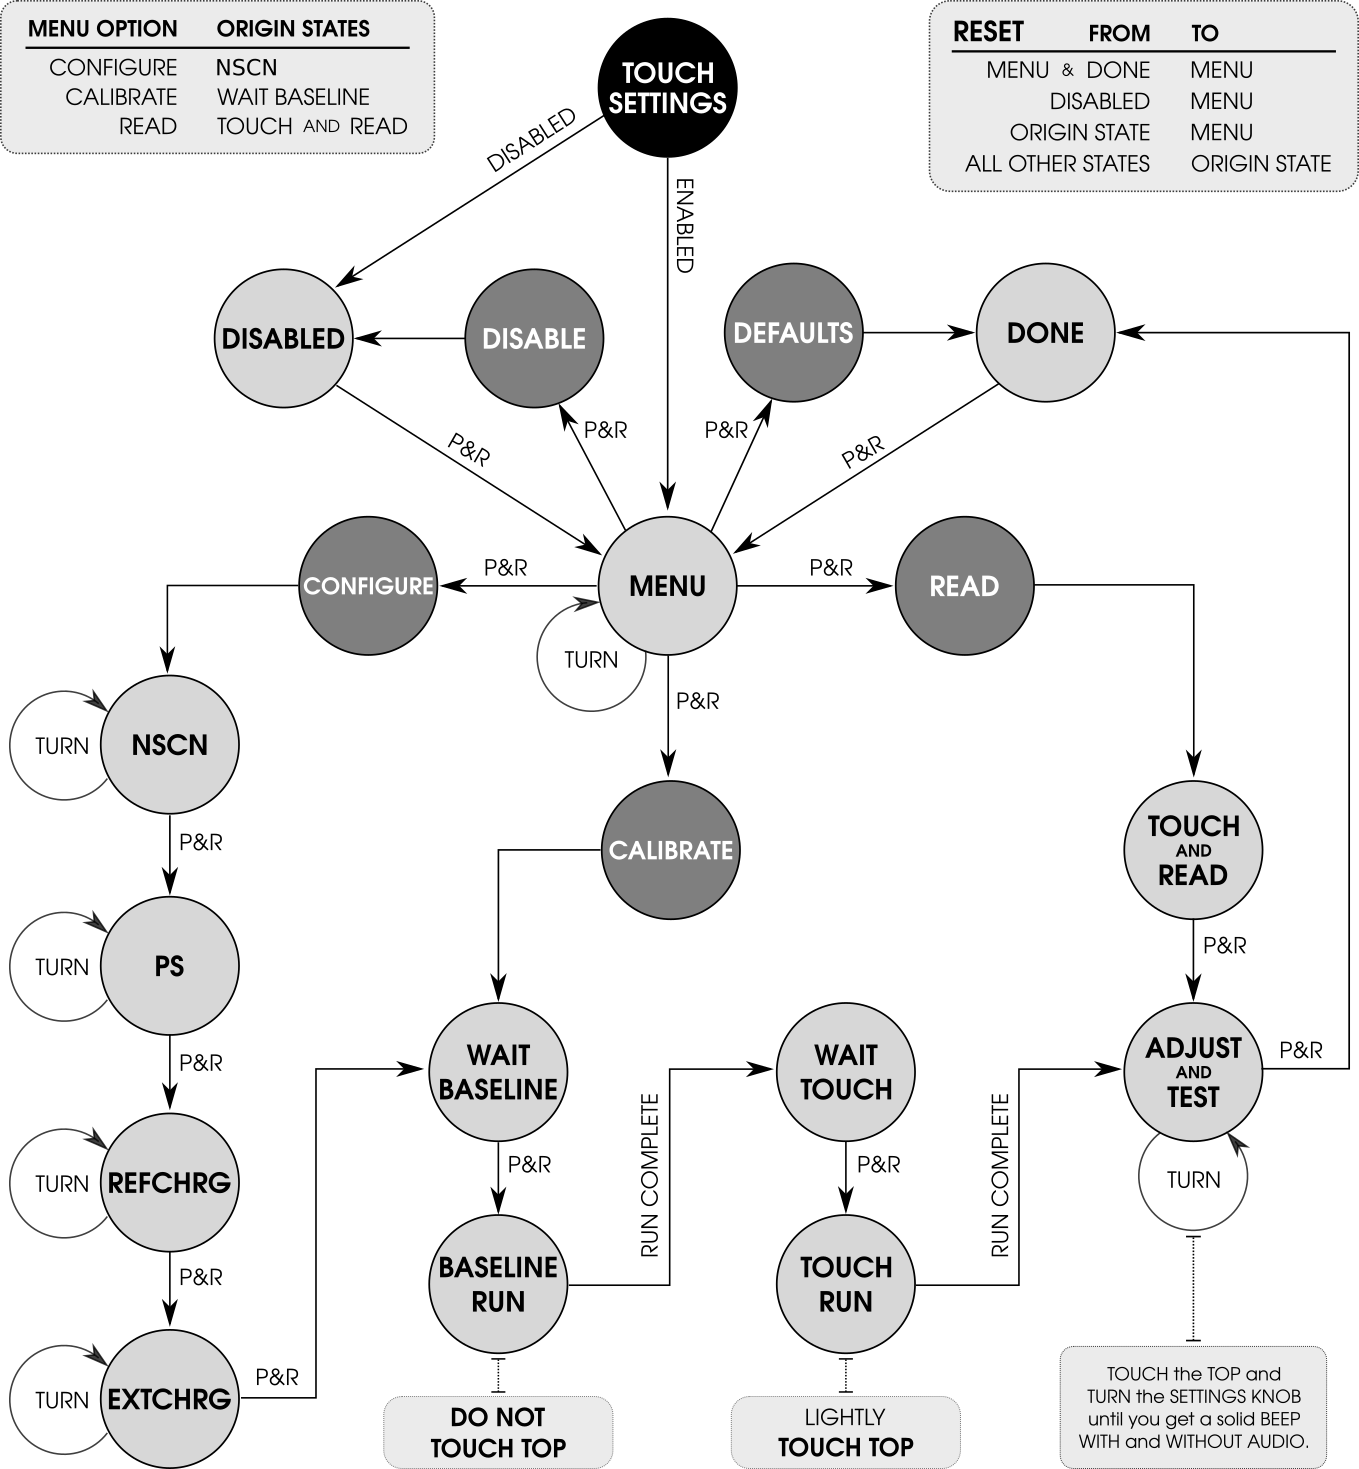
\includegraphics{images/touch_settings_state_diagram.png}
\caption{Touch Settings - State Diagram}
\end{figure}
